\documentclass[a4paper,10.5pt]{ltjsarticle}
\usepackage{graphicx}
\usepackage{graphics}
\usepackage{luatexja-fontspec}
\usepackage{caption}
\usepackage{amsmath,amssymb,bm,braket}
\usepackage{gnuplot-lua-tikz}
\usepackage[top=10truemm,bottom=15truemm,left=10truemm,right=10truemm]{geometry}
\usepackage{array}
\usepackage{upgreek}
\usepackage{fancyhdr}
\renewcommand{\refname}{}
\captionsetup[figure]{format=plain, labelformat=simple, labelsep=quad, font=bf}
\captionsetup[table]{format=plain, labelformat=simple, labelsep=quad, font=bf}
\parindent = 0pt
\setmainjfont[BoldFont=HiraMinProN-W6]{HiraMinPro-W3}
%[BoldFont=HGSMinchoE]{MSMincho}[BoldFont=HiraMinProN-W6]{HiraMinPro-W3}
\begin{document}
\centerline{\huge \bfseries 物理情報工学CD実験 報告書}
\centerline{ }
\rightline{\vspace{-3mm} \Large 2023年度   }
\begin{table}[h]
  \newcolumntype{I}{!{\vrule width 1.5pt}}
  \newcolumntype{i}{!{\vrule width 0.8pt}}
  \arrayrulewidth=0.8pt
  \renewcommand{\arraystretch}{1.5}
  \newcommand{\bhline}[1]{\noalign{\hrule height #1}}
  \huge
  \centering
  \begin{tabular}{Iwc{6cm}Iwc{2cm}iciwc{5cm}I}
    \bhline{1.5pt}
    実験テーマ&\multicolumn{3}{cI}{B4 強誘電体の特性と相転移}\\
    \hline
    担当教員名&\multicolumn{3}{cI}{劉TA}\\
    \hline
    実験整理番号&80&実験者氏名&平井 優我\\
    \hline
    共同実験者氏名&\multicolumn{3}{cI}{肥田 侑真、日野 正一、松田 遥}\\
    \hline
    曜日組&木&実験日&10月26日\\
    \hline
    実験回&3&報告書提出日&10月30日\\
    \bhline{1.5pt}
  \end{tabular}
\end{table}
\clearpage
%1-2---------------------------------------------------------------------------
{\Large \bfseries 1.目的\\}
強誘電体メモリーとして実用化されている強誘電体材料の基礎物性を理解する。\\
\\
\leftline
{\Large \bfseries 2.実験方法}\linebreak
\leftline
{\large \bfseries 2.1市販コンデンサおよび$\mathrm{BaTiO_3}$試料の周波数特性の測定(実験1)}\linebreak
 市販コンデンサーをLCRメーターにつなぎ,所定の周波数値で室温での電気容量$C$を測定した。次に、誘電特性の温度変化測定用に作られた$\mathrm{BaTiO_3}$試料をLCRメーターにつなぎ、所定の周波数値で室温での電気容量$C$を測定した。このとき、$\mathrm{BaTiO_3}$試料は電気炉内に設置してあった。\\
\\
\leftline
{\large \bfseries 2.2室温(強誘電状態)での$\mathrm{BaTiO_3}$の$D-E$曲線の観察(実験2)}\linebreak
 $\mathrm{BaTiO_3}$試料に繋がれたLCRメーターからの両端子をはずし、図1に示す測定回路であるSawyer-Tower回路に繋ぎ替えた。そしてスライダックを過電流保護回路に接続した後、スライダックのつまみを回して50 Hzの電圧を90 Vまで印加した。そのときの$D-E$曲線に関するデータをデジタルオシロスコープで観察し、データをUSBに保存した
\begin{figure}[ht]
\centering
\includegraphics[scale=0.3]{figure1.eps}
\caption{Sawyer-Tower回路}
\end{figure}
\\
\leftline
{\large \bfseries 2.3 $\mathrm{BaTiO_3}$の温度変化(昇温時)における$D-E$曲線の測定(実験3)}\linebreak
 およそ30分かけて自動的に約$200\ ^\circ \mathrm{C}$まで昇温するように設定した温度コントロー
ラーを用いて、電気炉の温度をPID制御を行いながら昇温させた。そして、室温($T=23\ ^\circ \mathrm{C}$)\ 〜\ 約$200\ ^\circ \mathrm{C}$の各温度で$D-E$曲線に関するデータをデジタルオシロスコープで観察し、データをUSBに保存した。\\
\\
\leftline
{\large \bfseries 2.4常誘電状態での$\mathrm{BaTiO_3}$の$D-E$曲線の観察(実験4)}\linebreak
 $\mathrm{BaTiO_3}$試料が$200\ ^\circ \mathrm{C}$で一定となるように温度制御器を設定し、約$200\ ^\circ \mathrm{C}$での$D-E$曲線に関するデータをデジタルオシロスコープで観察し,データをUSBに保存した。\\
\\
\clearpage
%2-3-------------------------------------------------------------------
\leftline
{\large \bfseries 2.5常誘電状態での$D$対$E$のシミュレーションと各温度$T$における誘電損失$\tan{\delta}$の算出}
\leftline
{\large \bfseries \ \ \ \ \ (実験5)}
 印加電圧$E$に対する応答としての$D$の遅れを角度として入力すると、ディスプレイ上に楕円形の$D-E$曲線を得た。実験3で観察した常誘電状態での$D-E$曲線に関するデータから、各温度$T$における位相の遅れ角$\delta$を推定し、誘電損失$\tan{\delta}$を算出した。\\
\\
\leftline
{\large \bfseries 2.6相転移のシミュレーション(実験6)}
 昇温時において、測定温度$T\ [\mathrm{K}]$=399, 400, 401, 402, 403, 404, 405, 405.3, 406, 407, 407.2, 408, 409, 410, 411, 412のとき、分極$P$の関数として強誘電状態と常誘電状態の自由エネルギー差$\Delta F(P)$の$P ≥ 0$の領域をコンピューターによって観察した。次に降温時において、測定温度$T\ [\mathrm{K}]$=412, 411, 410, 409, 408, 407.2, 407, 406, 405.3, 405, 404, 403, 402, 401, 400, 399について降温時の相転移のシミュレーションし、結果を得た。\\
\\
\leftline
{\Large \bfseries 3.結果}\linebreak
\leftline
{\large \bfseries 3.1市販コンデンサおよび$\mathrm{BaTiO_3}$試料の周波数特性の測定(実験1)}\linebreak
 室温においてのそれぞれの周波数$f\ [\mathrm{Hz}]$に対する市販のコンデンサ、$\mathrm{BaTiO_3}$試料の電気容量$C_1,\ C_2 \ [\mathrm{nF}]$を表1に示す。

\begin{table}[h]
  \centering
  \caption{それぞれの周波数に対する市販のコンデンサー、$\mathrm{BaTiO_3}$試料の電気容量}
  \newcommand{\bhline}[1]{\noalign{\hrule height #1}}
  \newcolumntype{I}{!{\vrule width 1.5pt}}
  \begin{tabular}{Ic|ccI}
    \bhline{1.5pt}
    周波数$f\ \mathrm{Hz}$&市販コンデンサーの電気容量$C_1\ \mathrm{nF}$&$\mathrm{BaTiO_3}$試料のの電気容量$C_2\ \mathrm{nF}$\\
    \bhline{1.0pt}
    100 & 15.7 & $2.22\times 10^{-3}$\\
    1k & 15.7 & $4.10\times 10^{-3}$\\
    10k & 15.5 & $8.23\times 10^{-3}$\\
    100k & 15.3 & $1.43\times 10^{-2}$\\
    \bhline{1.5pt}
  \end{tabular}
\end{table}

{\large \bfseries 3.2室温(強誘電状態)での$\mathrm{BaTiO_3}$の$D-E$曲線の観察(実験2)}
 実験で得られた室温での$\mathrm{BaTiO_3}$の$D-E$曲線を図2に示す。
\begin{figure}[h]
  \centering
  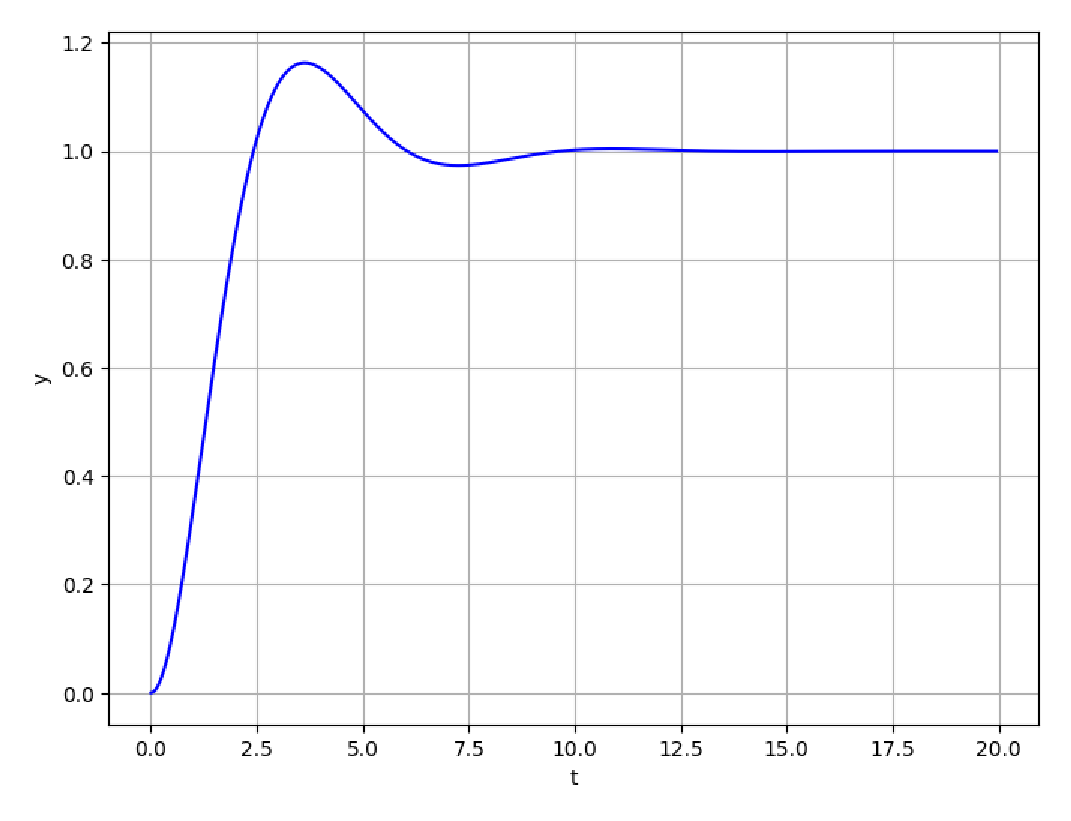
\includegraphics[scale=0.5]{figure2.eps}
  \caption{$D-E$曲線(室温)}
\end{figure}
\\
{\large \bfseries 3.3 $\mathrm{BaTiO_3}$の温度変化(昇温時)における$D-E$曲線の測定(実験3)}\\
 図3\ 〜\ 図12に昇温時における$D-E$曲線を示す。

\begin{figure}[htbp]
  \begin{minipage}[t]{0.30\linewidth}
    \centering
    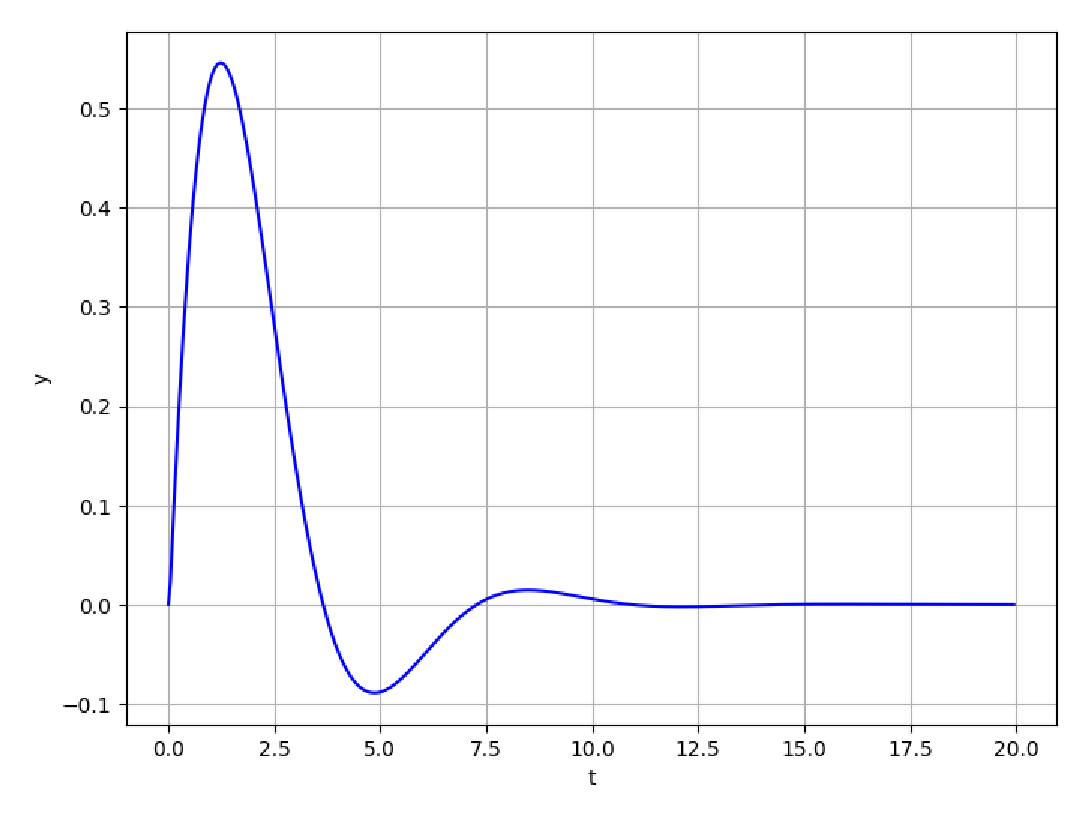
\includegraphics[keepaspectratio,scale=0.4]{figure3.eps}
    \caption{$D-E$曲線($T=40\ ^\circ \mathrm{C}$)}
  \end{minipage}
  \begin{minipage}[t]{0.30\linewidth}
    \centering
    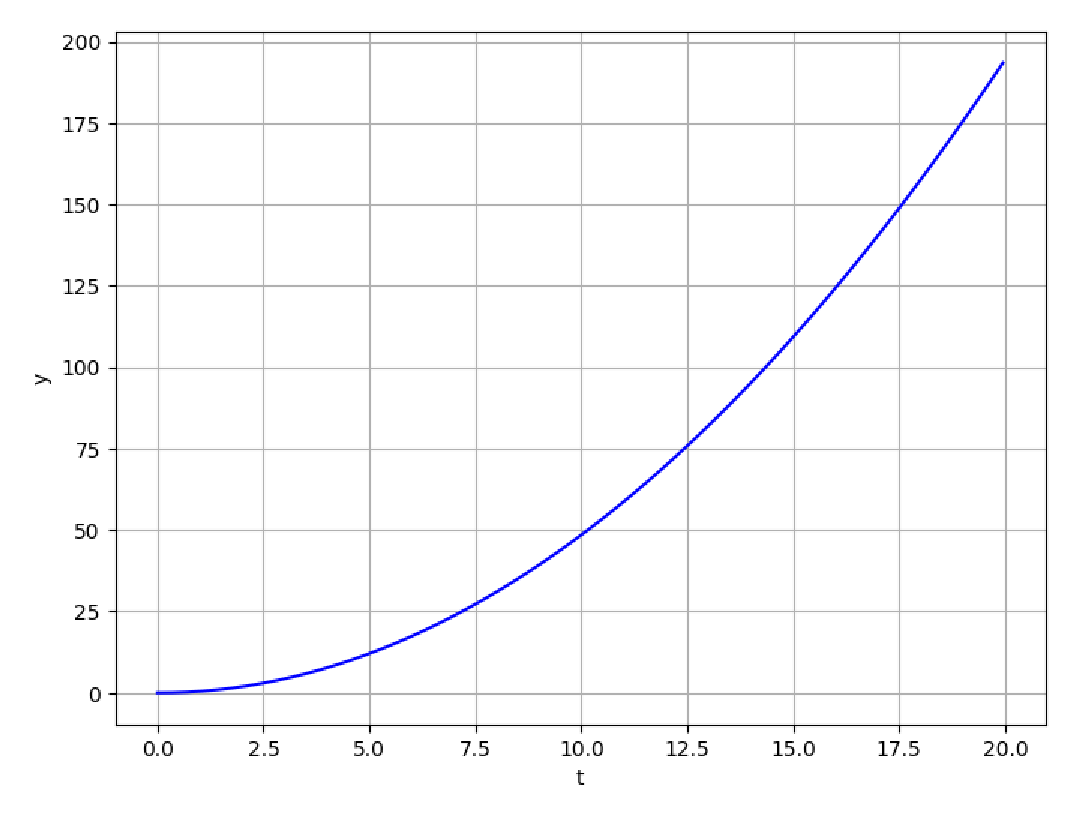
\includegraphics[keepaspectratio,scale=0.4]{figure4.eps}
    \caption{$D-E$曲線($T=60\ ^\circ \mathrm{C}$)}
  \end{minipage}
  \begin{minipage}[t]{0.30\linewidth}
    \centering
    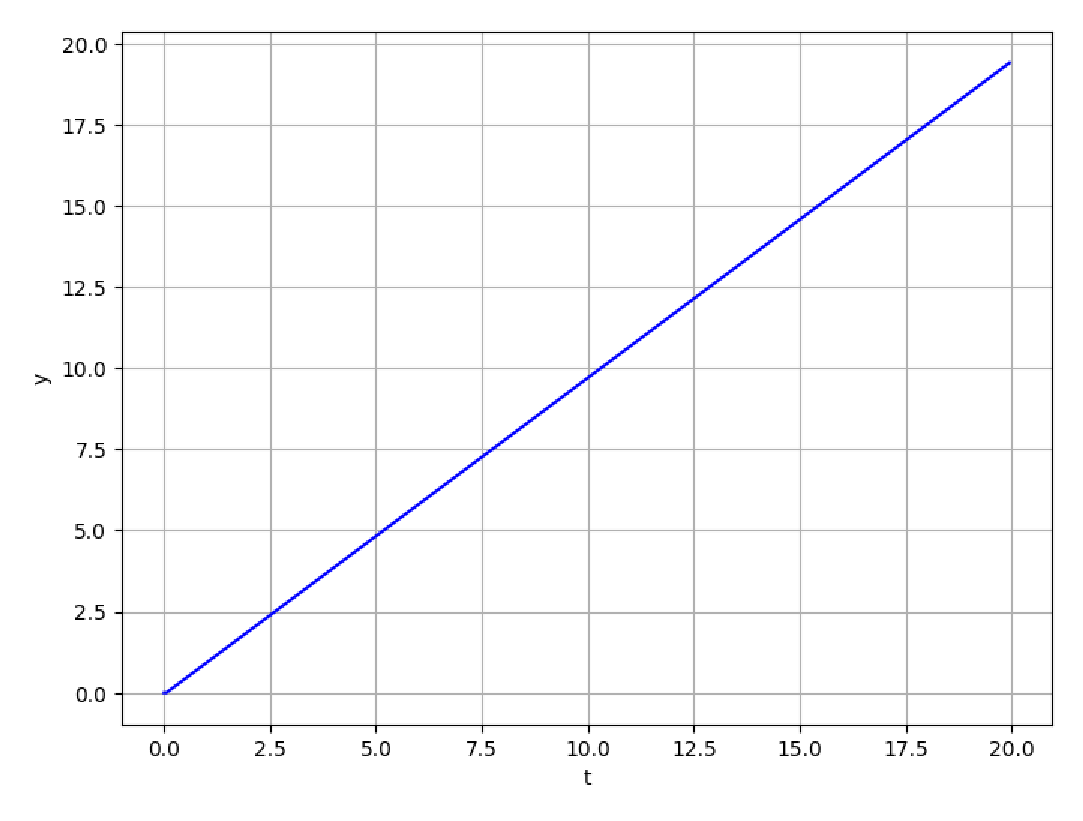
\includegraphics[keepaspectratio,scale=0.4]{figure5.eps}
    \caption{$D-E$曲線($T=80\ ^\circ \mathrm{C}$)}
  \end{minipage}

  \begin{minipage}[t]{0.30\linewidth}
    \centering
    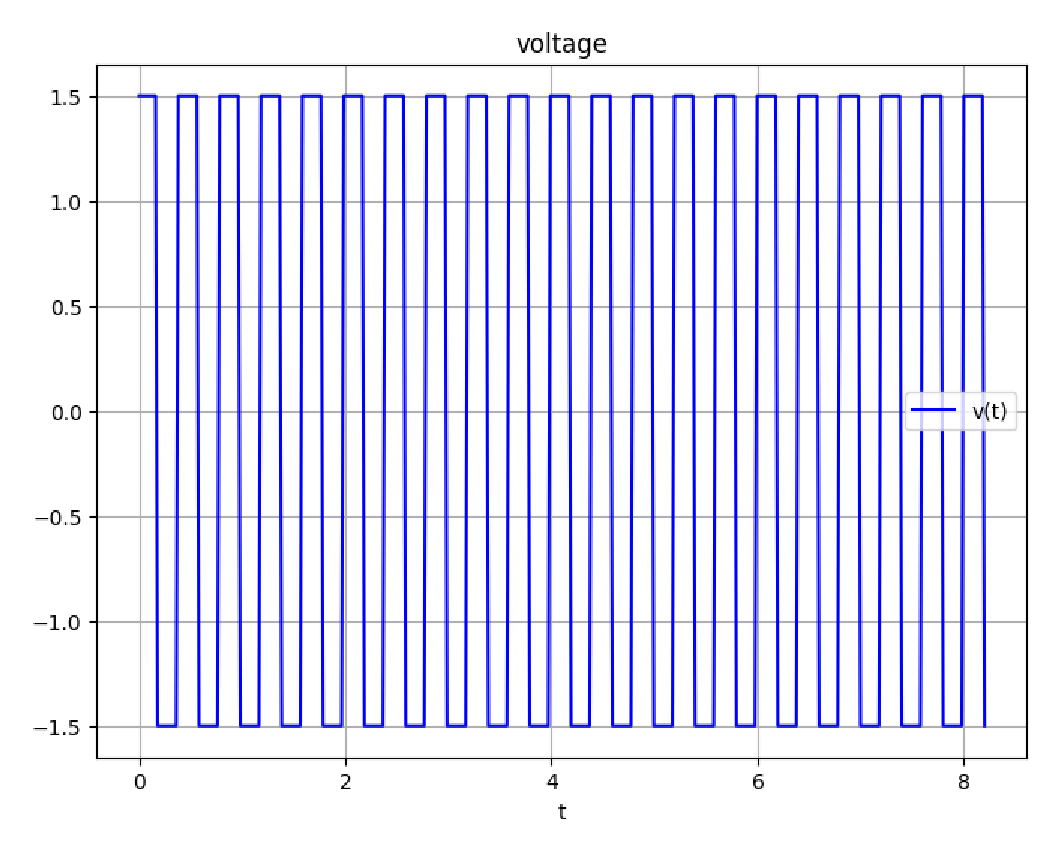
\includegraphics[keepaspectratio,scale=0.4]{figure6.eps}
    \caption{$D-E$曲線($T=100\ ^\circ \mathrm{C}$)}
  \end{minipage}
  \begin{minipage}[t]{0.30\linewidth}
    \centering
    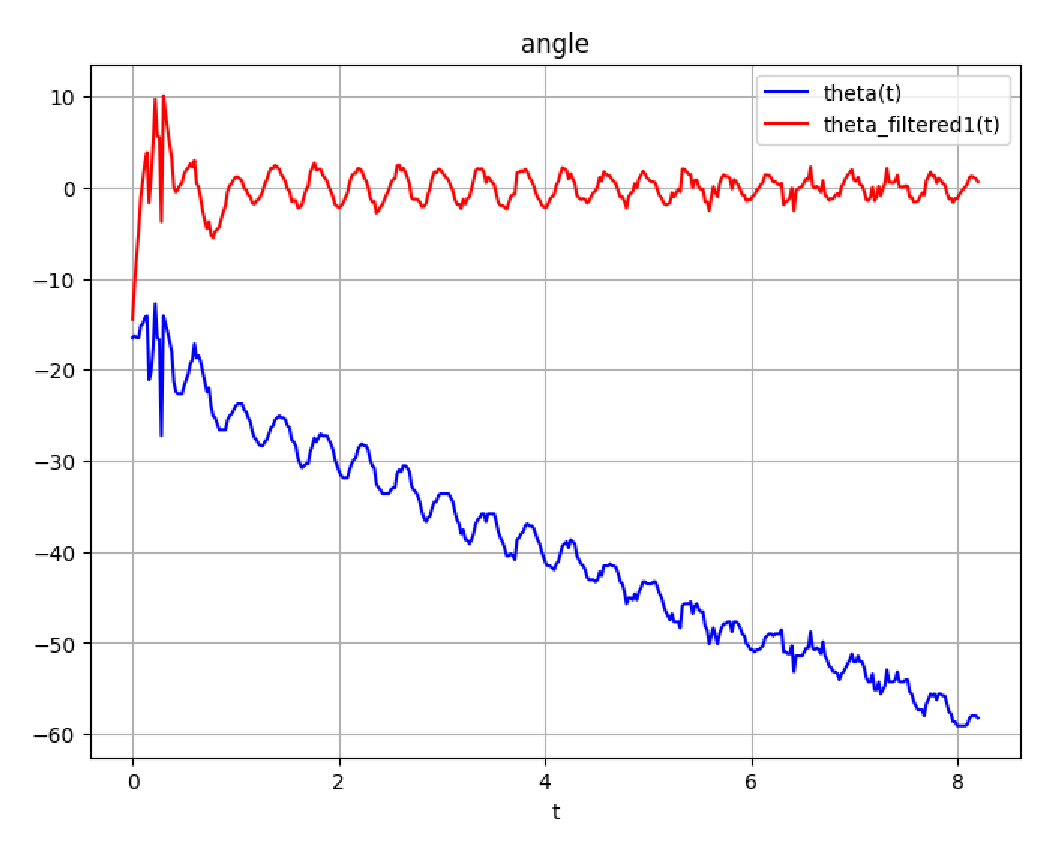
\includegraphics[keepaspectratio,scale=0.4]{figure7.eps}
    \caption{$D-E$曲線($T=120\ ^\circ \mathrm{C}$)}
  \end{minipage}
  \begin{minipage}[t]{0.30\linewidth}
    \centering
    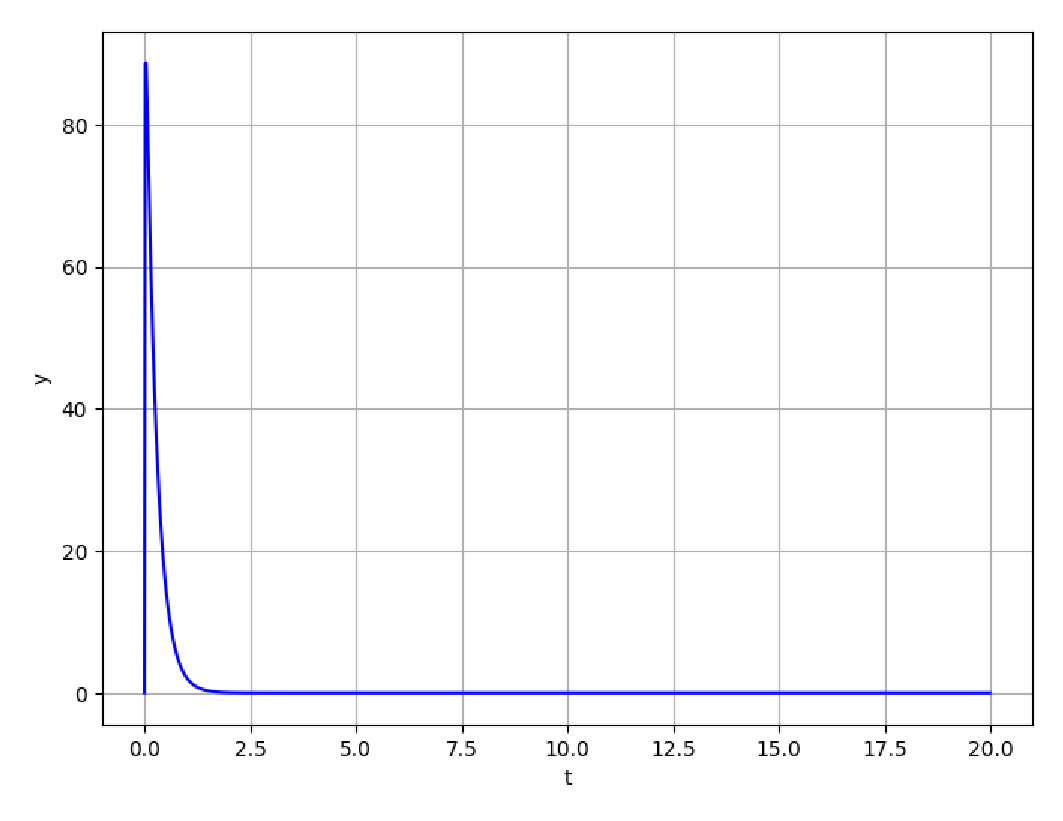
\includegraphics[keepaspectratio,scale=0.4]{figure8.eps}
    \caption{$D-E$曲線($T=125\ ^\circ \mathrm{C}$)}
  \end{minipage}

  \begin{minipage}[t]{0.30\linewidth}
    \centering
    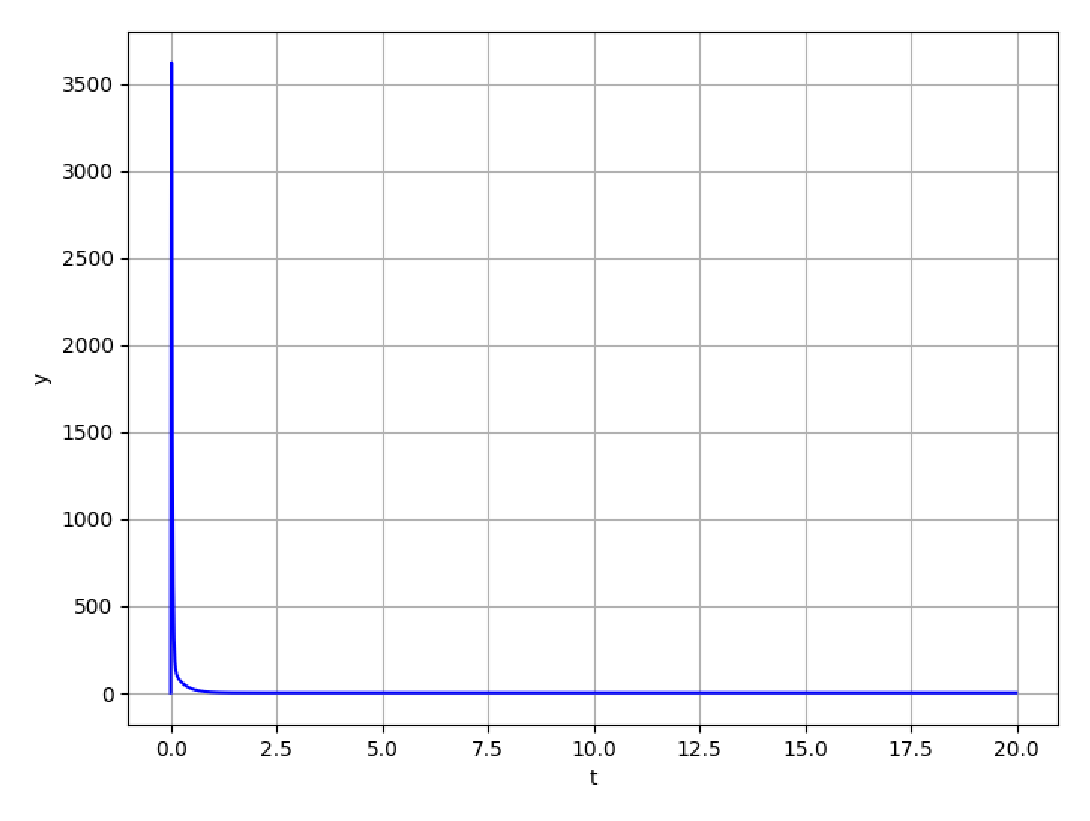
\includegraphics[keepaspectratio,scale=0.4]{figure9.eps}
    \caption{$D-E$曲線($T=130\ ^\circ \mathrm{C}$)}
  \end{minipage}
  \begin{minipage}[t]{0.30\linewidth}
    \centering
    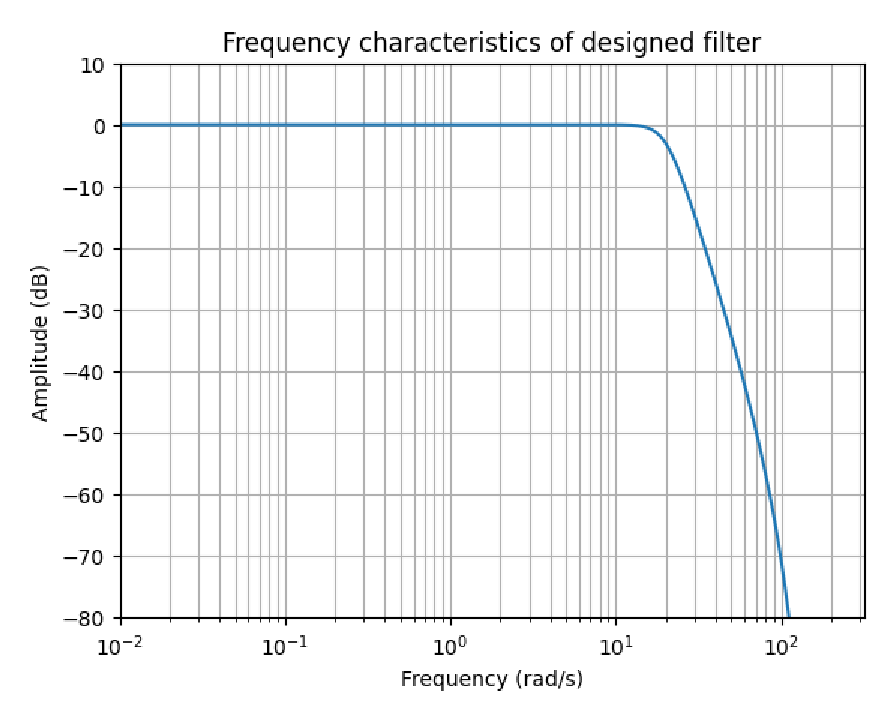
\includegraphics[keepaspectratio,scale=0.4]{figure10.eps}
    \caption{$D-E$曲線($T=135\ ^\circ \mathrm{C}$)}
  \end{minipage}
  \begin{minipage}[t]{0.30\linewidth}
    \centering
    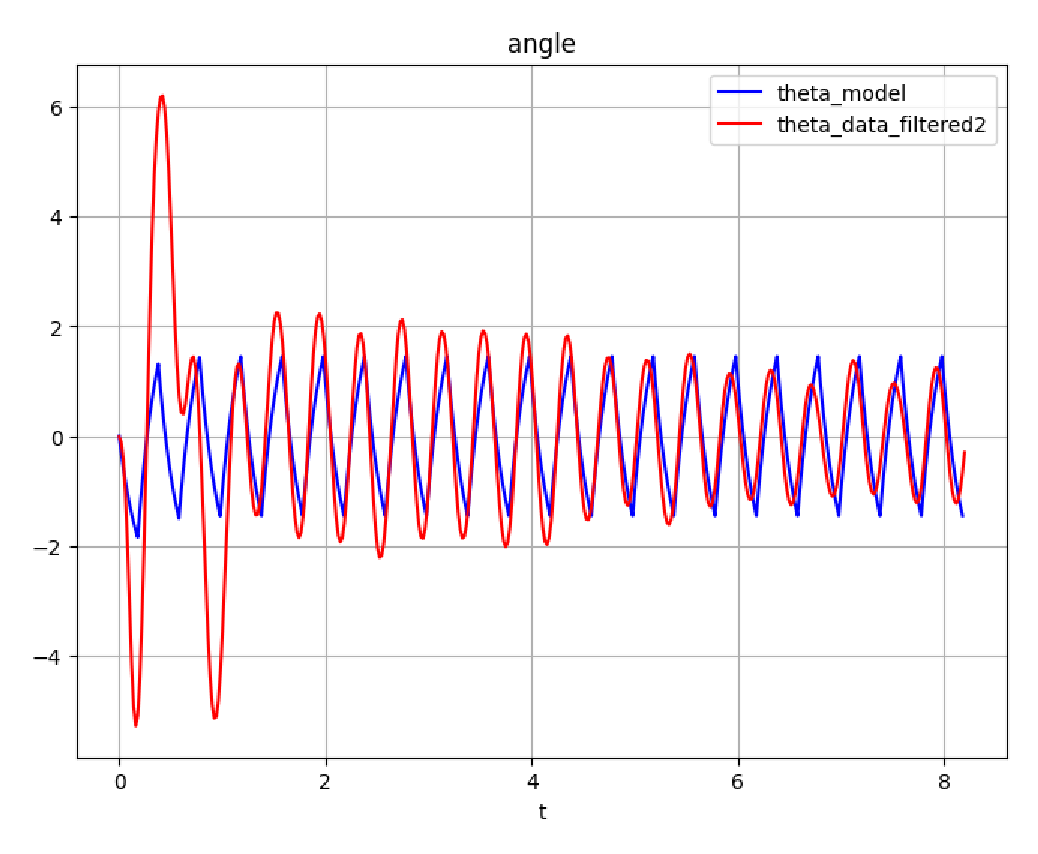
\includegraphics[keepaspectratio,scale=0.4]{figure11.eps}
    \caption{$D-E$曲線($T=140\ ^\circ \mathrm{C}$)}
  \end{minipage}

  \begin{minipage}[t]{0.30\linewidth}
    \centering
    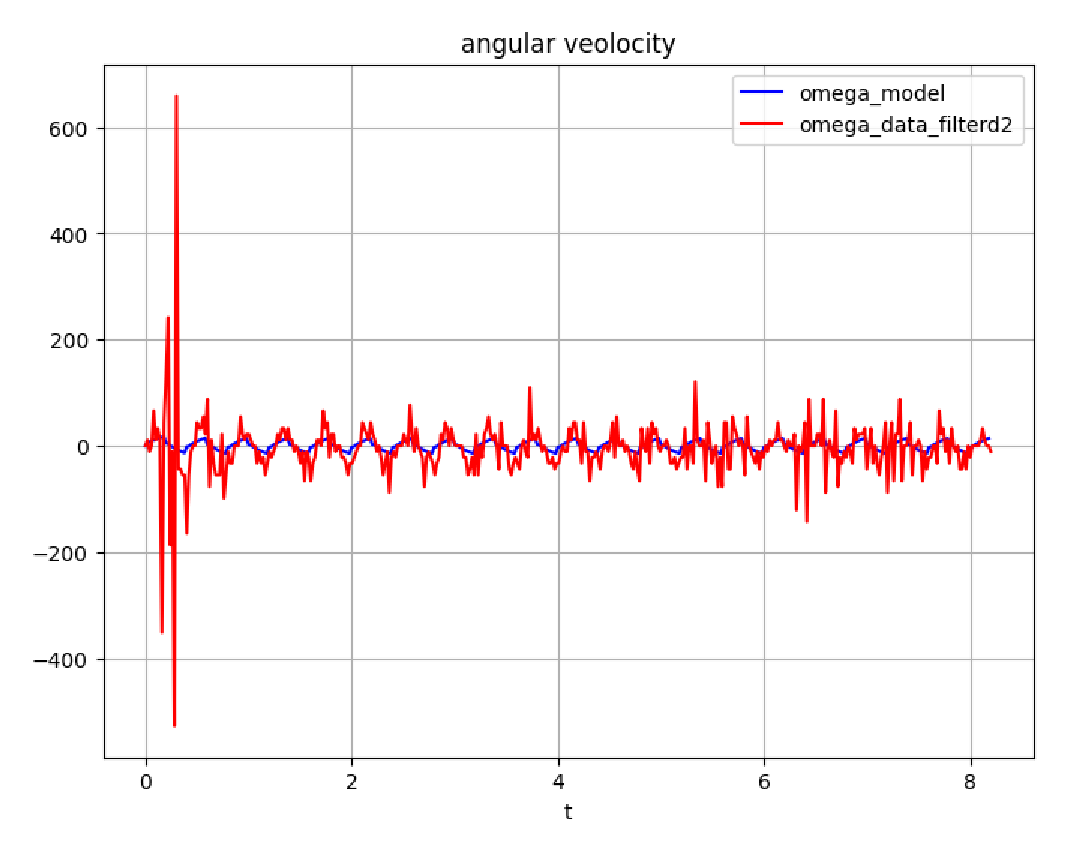
\includegraphics[keepaspectratio,scale=0.4]{figure12.eps}
    \caption{$D-E$曲線($T=160\ ^\circ \mathrm{C}$)}
  \end{minipage}
\end{figure}
\clearpage
%4-5---------------------------------------------------------------------------
{\large \bfseries 3.4常誘電状態での$\mathrm{BaTiO_3}$の$D-E$曲線の観察(実験4)}\\
実験で得られた温度$T=190\ ^\circ \mathrm{C}$での$\mathrm{BaTiO_3}$の$D-E$曲線を図3に示す。
\begin{figure}[h]
  \centering
  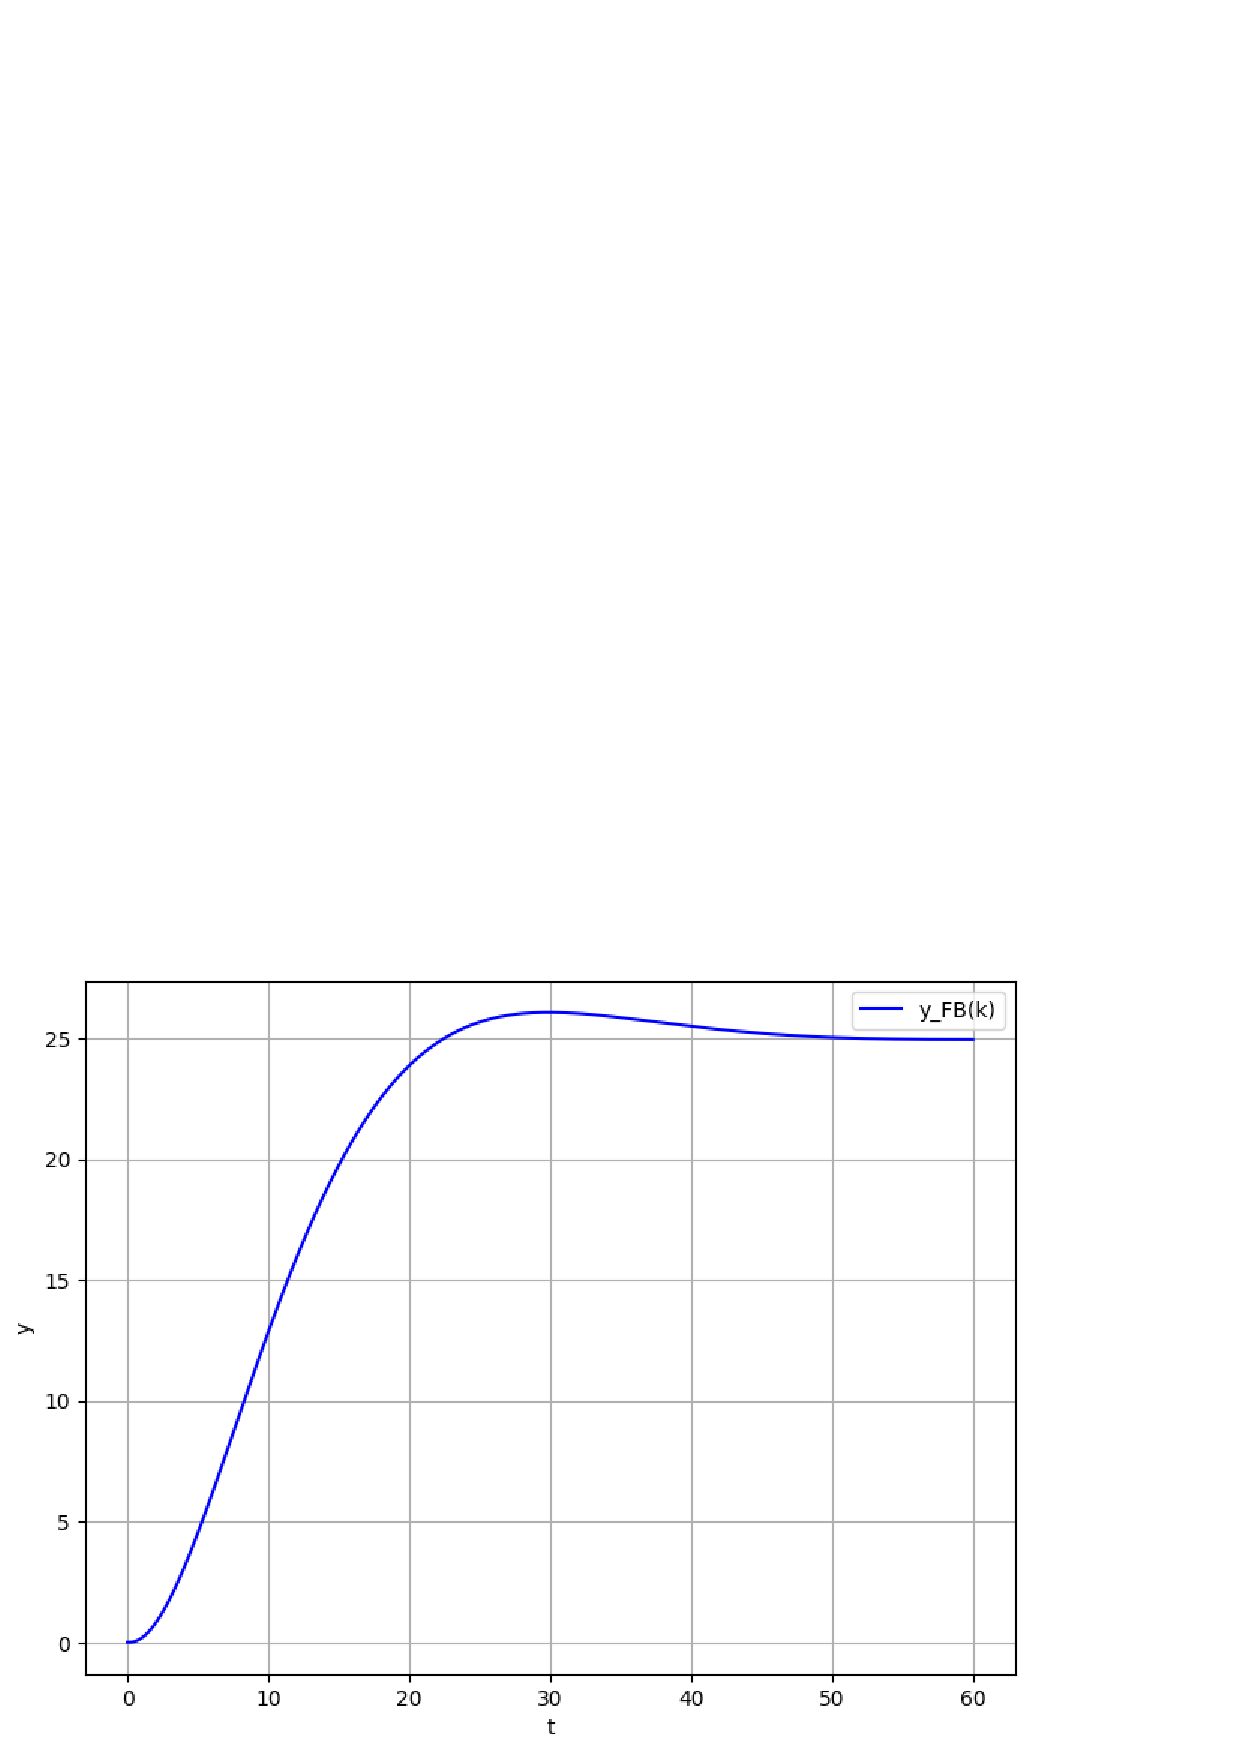
\includegraphics[scale=0.5]{figure13.png}
  \caption{$D-E$曲線($T=190\ ^\circ \mathrm{C}$)}
\end{figure}
\\
{\large \bfseries 3.5常誘電状態での$D$対$E$のシミュレーションと各温度$T$における誘電損失$\tan{\delta}$の算出}\\
 シミュレーションによって得られたフィッティング結果を図14\ 〜\ 図25に示す。

\begin{figure}[htbp]
  \begin{minipage}[h]{0.50\linewidth}
    \centering
    \includegraphics[keepaspectratio,scale=0.4]{figure14-1.eps}
  \end{minipage}
  \begin{minipage}[h]{0.50\linewidth}
    \centering
    \includegraphics[keepaspectratio,scale=0.4]{figure14-2.eps}
  \end{minipage}
  \caption{$V_\mathrm{in},\ V_\mathrm{out}$のフィッティング(室温)}
\end{figure}

\begin{figure}[htbp]
  \begin{minipage}[h]{0.50\linewidth}
    \centering
    \includegraphics[keepaspectratio,scale=0.4]{figure15-1.eps}
  \end{minipage}
  \begin{minipage}[h]{0.50\linewidth}
    \centering
    \includegraphics[keepaspectratio,scale=0.4]{figure15-2.eps}
  \end{minipage}
  \caption{$V_\mathrm{in},\ V_\mathrm{out}$のフィッティング($T=40\ ^\circ \mathrm{C}$)}
\end{figure}
\clearpage
%------------------------------------------------------------------------------
\begin{figure}[b]
  \begin{minipage}[h]{0.50\linewidth}
    \centering
    \includegraphics[keepaspectratio,scale=0.4]{figure16-1.eps}
  \end{minipage}
  \begin{minipage}[h]{0.50\linewidth}
    \centering
    \includegraphics[keepaspectratio,scale=0.4]{figure16-2.eps}
  \end{minipage}
  \caption{$V_\mathrm{in},\ V_\mathrm{out}$のフィッティング($T=60\ ^\circ \mathrm{C}$)}
\end{figure}

\begin{figure}[b]
  \begin{minipage}[h]{0.50\linewidth}
    \centering
    \includegraphics[keepaspectratio,scale=0.4]{figure17-1.eps}
  \end{minipage}
  \begin{minipage}[h]{0.50\linewidth}
    \centering
    \includegraphics[keepaspectratio,scale=0.4]{figure17-2.eps}
  \end{minipage}
  \caption{$V_\mathrm{in},\ V_\mathrm{out}$のフィッティング($T=80\ ^\circ \mathrm{C}$)}
\end{figure}

\begin{figure}[b]
  \begin{minipage}[h]{0.50\linewidth}
    \centering
    \includegraphics[keepaspectratio,scale=0.4]{figure18-1.eps}
  \end{minipage}
  \begin{minipage}[h]{0.50\linewidth}
    \centering
    \includegraphics[keepaspectratio,scale=0.4]{figure18-2.eps}
  \end{minipage}
  \caption{$V_\mathrm{in},\ V_\mathrm{out}$のフィッティング($T=100\ ^\circ \mathrm{C}$)}
\end{figure}

\begin{figure}[b]
  \begin{minipage}[h]{0.50\linewidth}
    \centering
    \includegraphics[keepaspectratio,scale=0.4]{figure19-1.eps}
  \end{minipage}
  \begin{minipage}[h]{0.50\linewidth}
    \centering
    \includegraphics[keepaspectratio,scale=0.4]{figure19-2.eps}
  \end{minipage}
  \caption{$V_\mathrm{in},\ V_\mathrm{out}$のフィッティング($T=120\ ^\circ \mathrm{C}$)}
\end{figure}
\clearpage
%6-7---------------------------------------------------------------------------
\begin{figure}[b]
  \begin{minipage}[h]{0.50\linewidth}
    \centering
    \includegraphics[keepaspectratio,scale=0.4]{figure20-1.eps}
  \end{minipage}
  \begin{minipage}[h]{0.50\linewidth}
    \centering
    \includegraphics[keepaspectratio,scale=0.4]{figure20-2.eps}
  \end{minipage}
  \caption{$V_\mathrm{in},\ V_\mathrm{out}$のフィッティング($T=125\ ^\circ \mathrm{C}$)}
\end{figure}

\begin{figure}[b]
  \begin{minipage}[h]{0.50\linewidth}
    \centering
    \includegraphics[keepaspectratio,scale=0.4]{figure21-1.eps}
  \end{minipage}
  \begin{minipage}[h]{0.50\linewidth}
    \centering
    \includegraphics[keepaspectratio,scale=0.4]{figure21-2.eps}
  \end{minipage}
  \caption{$V_\mathrm{in},\ V_\mathrm{out}$のフィッティング($T=130\ ^\circ \mathrm{C}$)}
\end{figure}

\begin{figure}[b]
  \begin{minipage}[h]{0.50\linewidth}
    \centering
    \includegraphics[keepaspectratio,scale=0.4]{figure22-1.eps}
  \end{minipage}
  \begin{minipage}[h]{0.50\linewidth}
    \centering
    \includegraphics[keepaspectratio,scale=0.4]{figure22-2.eps}
  \end{minipage}
  \caption{$V_\mathrm{in},\ V_\mathrm{out}$のフィッティング($T=135\ ^\circ \mathrm{C}$)}
\end{figure}

\begin{figure}[b]
  \begin{minipage}[h]{0.50\linewidth}
    \centering
    \includegraphics[keepaspectratio,scale=0.4]{figure23-1.eps}
  \end{minipage}
  \begin{minipage}[h]{0.50\linewidth}
    \centering
    \includegraphics[keepaspectratio,scale=0.4]{figure23-2.eps}
  \end{minipage}
  \caption{$V_\mathrm{in},\ V_\mathrm{out}$のフィッティング($T=140\ ^\circ \mathrm{C}$)}
\end{figure}
\clearpage
%7-8----------------------------------------------------------------------------
\begin{figure}[htbp]
  \begin{minipage}[h]{0.50\linewidth}
    \centering
    \includegraphics[keepaspectratio,scale=0.4]{figure24-1.eps}
  \end{minipage}
  \begin{minipage}[h]{0.50\linewidth}
    \centering
    \includegraphics[keepaspectratio,scale=0.4]{figure24-2.eps}
  \end{minipage}
  \caption{$V_\mathrm{in},\ V_\mathrm{out}$のフィッティング($T=160\ ^\circ \mathrm{C}$)}
\end{figure}

\begin{figure}[h]
  \begin{minipage}[h]{0.50\linewidth}
    \centering
    \includegraphics[keepaspectratio,scale=0.4]{figure25-1.eps}
  \end{minipage}
  \begin{minipage}[h]{0.50\linewidth}
    \centering
    \includegraphics[keepaspectratio,scale=0.4]{figure25-2.eps}
  \end{minipage}
  \caption{$V_\mathrm{in},\ V_\mathrm{out}$のフィッティング($T=190\ ^\circ \mathrm{C}$)}
\end{figure}
また、表2にそれぞれの温度$T$で得られた遅れ$\delta$と誘電損失$\tan{\delta}$を示す。
\begin{table}[h]
  \centering
  \newcommand{\bhline}[1]{\noalign{\hrule height #1}}
  \newcolumntype{I}{!{\vrule width 1.5pt}}
  \caption{それぞれの温度$T$での遅れ$\delta$と誘電損失$\tan{\delta}$}
  \begin{tabular}{Ic|ccI}
    \bhline{1.5pt}
    温度$T\ /\ \mathrm{K}$&遅れ$\delta \ /\ \mathrm{rad}$&誘電損失$\tan{\delta}$\\
    \bhline{1.0pt}
    40	& 3.23 &	0.0907\\
    60	& 3.25 &	0.105\\
    80	& 3.26 &	0.124\\
    100	& 0.207 &	0.211\\
    120	& 0.325 &	0.336\\
    125	& 0.469 &	0.507\\
    130	& 3.29	& 0.148\\
    135	& 3.26 &	0.118\\
    140	& 3.25 &	0.108\\
    160	& 3.25 &	0.107\\
    190	& 3.26 &	0.116\\
    \bhline{1.5pt}
  \end{tabular}
\end{table}
\clearpage
%8-9----------------------------------------------------------------------------
{\large \bfseries 3.6相転移のシミュレーション(実験6)}\\
 図1、図2に昇温時、降温時の相転移シミュレーションの結果を示す。

\begin{figure}[h]
  \centering
  \includegraphics[keepaspectratio,scale=0.25]{figure26.eps}
  \caption{昇温時}
\end{figure}

\begin{figure}[h]
  \centering
  \includegraphics[keepaspectratio,scale=0.25]{figure27.eps}
  \caption{降温時}
\end{figure}
\clearpage
%9-10---------------------------------------------------------------------------
{\Large \bfseries 4.考察}\\
{\large \bfseries 4.1誘電体の$D-E$曲線の測定原理}
\begin{figure}[h]
  \centering
  \includegraphics[keepaspectratio,scale=0.30]{figure28.eps}
  \caption{Sawyer-Tower回路}
\end{figure}
\\
 Sawyer-Tower回路によってどのようにして誘電体のD-E曲線が測定されるかを説明する。図28から、$R_2$と$R_3$の抵抗値の比から、誘電体と$R_3$をつなぐ導線の電圧は$11X_\mathrm{high}-10X_\mathrm{low}$となる。よって、誘電体の電圧$V$は

\begin{displaymath}
  V=11X_\mathrm{high}-10X_\mathrm{low}-Y_\mathrm{high}
\end{displaymath}

となる。よって、$C$の電極間の距離を$d$とすれば、

\begin{displaymath}
  E=\frac{V}{d}=\frac{11X_\mathrm{high}-10X_\mathrm{low}-Y_\mathrm{high}}{d}
\end{displaymath}

となる。また、$R_1$、オシロスコープの抵抗値は十分に大きく、それらに流れる電流は無視することができる。このことから、$C$に貯まる電気量$Q$と$Q_0$等しい。よって、

\begin{displaymath}
  Q=Q_0=C_0(Y_\mathrm{high}-Y_\mathrm{low})
\end{displaymath}

となり、$Q=CV$の関係と電極の面積Sから、

\begin{displaymath}
  D=\frac{Q}{S}=\frac{C_0(Y_\mathrm{high}-Y_\mathrm{low})}{S}
\end{displaymath}

となる。これより、Sawyer-Tower回路によって、$D$と$E$を測定することができる。
\clearpage
%10-11--------------------------------------------------------------------------
{\large \bfseries 4.3Landauモデルによる相転移シミュレーションの説明}\\
 物質の状態変化について、分極$P$を秩序度して自由エネルギ$F$を$P$の展開形式で論じるモデルをLandauのモデルという。ここで、参考文献の\cite{text}の(49)式より、変化量$\Delta F$は、

\begin{displaymath}
  \Delta F=A_1(T-T_0)P^2+A_2P^4+A_3P^6
\end{displaymath}

と表せる。ここで、$A_1>0,A_2<0,A_3>0$ と置くことによって実験結果をよく記述できる。\\
\\
{\large \bfseries 4.4強誘電体$\mathrm{BaTiO_3}$の誘電損失$\tan{\delta}$の温度依存性}\\
 図29に強誘電体$\mathrm{BaTiO_3}$の誘電損失$\tan{\delta}$の温度依存性のグラフを示す。

\begin{figure}[h]
  \centering
  \scalebox{0.7}[0.7]{
\begin{tikzpicture}[gnuplot]
%% generated with GNUPLOT 5.4p10 (Lua 5.4; terminal rev. Jun 2020, script rev. 118)
%% Thu Nov  2 15:24:43 2023
\path (0.000,0.000) rectangle (12.500,8.750);
\gpcolor{color=gp lt color border}
\gpsetlinetype{gp lt border}
\gpsetdashtype{gp dt solid}
\gpsetlinewidth{1.00}
\draw[gp path] (0.018,0.031)--(0.198,0.031);
\draw[gp path] (12.480,0.031)--(12.300,0.031);
\node[gp node right] at (-0.166,0.031) {$0.05$};
\draw[gp path] (0.018,0.900)--(0.198,0.900);
\draw[gp path] (12.480,0.900)--(12.300,0.900);
\node[gp node right] at (-0.166,0.900) {$0.1$};
\draw[gp path] (0.018,1.768)--(0.198,1.768);
\draw[gp path] (12.480,1.768)--(12.300,1.768);
\node[gp node right] at (-0.166,1.768) {$0.15$};
\draw[gp path] (0.018,2.637)--(0.198,2.637);
\draw[gp path] (12.480,2.637)--(12.300,2.637);
\node[gp node right] at (-0.166,2.637) {$0.2$};
\draw[gp path] (0.018,3.506)--(0.198,3.506);
\draw[gp path] (12.480,3.506)--(12.300,3.506);
\node[gp node right] at (-0.166,3.506) {$0.25$};
\draw[gp path] (0.018,4.375)--(0.198,4.375);
\draw[gp path] (12.480,4.375)--(12.300,4.375);
\node[gp node right] at (-0.166,4.375) {$0.3$};
\draw[gp path] (0.018,5.243)--(0.198,5.243);
\draw[gp path] (12.480,5.243)--(12.300,5.243);
\node[gp node right] at (-0.166,5.243) {$0.35$};
\draw[gp path] (0.018,6.112)--(0.198,6.112);
\draw[gp path] (12.480,6.112)--(12.300,6.112);
\node[gp node right] at (-0.166,6.112) {$0.4$};
\draw[gp path] (0.018,6.981)--(0.198,6.981);
\draw[gp path] (12.480,6.981)--(12.300,6.981);
\node[gp node right] at (-0.166,6.981) {$0.45$};
\draw[gp path] (0.018,7.849)--(0.198,7.849);
\draw[gp path] (12.480,7.849)--(12.300,7.849);
\node[gp node right] at (-0.166,7.849) {$0.5$};
\draw[gp path] (0.018,8.718)--(0.198,8.718);
\draw[gp path] (12.480,8.718)--(12.300,8.718);
\node[gp node right] at (-0.166,8.718) {$0.55$};
\draw[gp path] (0.751,0.031)--(0.751,0.211);
\draw[gp path] (0.751,8.718)--(0.751,8.538);
\node[gp node center] at (0.751,-0.277) {$40$};
\draw[gp path] (2.217,0.031)--(2.217,0.211);
\draw[gp path] (2.217,8.718)--(2.217,8.538);
\node[gp node center] at (2.217,-0.277) {$60$};
\draw[gp path] (3.683,0.031)--(3.683,0.211);
\draw[gp path] (3.683,8.718)--(3.683,8.538);
\node[gp node center] at (3.683,-0.277) {$80$};
\draw[gp path] (5.149,0.031)--(5.149,0.211);
\draw[gp path] (5.149,8.718)--(5.149,8.538);
\node[gp node center] at (5.149,-0.277) {$100$};
\draw[gp path] (6.616,0.031)--(6.616,0.211);
\draw[gp path] (6.616,8.718)--(6.616,8.538);
\node[gp node center] at (6.616,-0.277) {$120$};
\draw[gp path] (8.082,0.031)--(8.082,0.211);
\draw[gp path] (8.082,8.718)--(8.082,8.538);
\node[gp node center] at (8.082,-0.277) {$140$};
\draw[gp path] (9.548,0.031)--(9.548,0.211);
\draw[gp path] (9.548,8.718)--(9.548,8.538);
\node[gp node center] at (9.548,-0.277) {$160$};
\draw[gp path] (11.014,0.031)--(11.014,0.211);
\draw[gp path] (11.014,8.718)--(11.014,8.538);
\node[gp node center] at (11.014,-0.277) {$180$};
\draw[gp path] (12.480,0.031)--(12.480,0.211);
\draw[gp path] (12.480,8.718)--(12.480,8.538);
\node[gp node center] at (12.480,-0.277) {$200$};
\draw[gp path] (0.018,8.718)--(0.018,0.031)--(12.480,0.031)--(12.480,8.718)--cycle;
\node[gp node center,rotate=-270] at (-1.194,4.374) {誘電損失$\ \tan{\delta}$};
\node[gp node center] at (6.249,-0.738) {温度$T\ /\ \mathrm{K}$};
\gpcolor{rgb color={0.000,0.000,0.000}}
\gpsetlinewidth{5.00}
\draw[gp path] (0.751,0.738)--(2.217,0.987)--(3.683,1.317)--(5.149,2.828)--(6.616,5.000)%
  --(6.982,7.971)--(7.349,1.734)--(7.715,1.212)--(8.082,1.039)--(9.548,1.021)--(11.747,1.178);
\gpsetpointsize{3.20}
\gp3point{gp mark 7}{}{(0.751,0.738)}
\gp3point{gp mark 7}{}{(2.217,0.987)}
\gp3point{gp mark 7}{}{(3.683,1.317)}
\gp3point{gp mark 7}{}{(5.149,2.828)}
\gp3point{gp mark 7}{}{(6.616,5.000)}
\gp3point{gp mark 7}{}{(6.982,7.971)}
\gp3point{gp mark 7}{}{(7.349,1.734)}
\gp3point{gp mark 7}{}{(7.715,1.212)}
\gp3point{gp mark 7}{}{(8.082,1.039)}
\gp3point{gp mark 7}{}{(9.548,1.021)}
\gp3point{gp mark 7}{}{(11.747,1.178)}
\gpcolor{color=gp lt color border}
\gpsetlinewidth{1.00}
\draw[gp path] (0.018,8.718)--(0.018,0.031)--(12.480,0.031)--(12.480,8.718)--cycle;
%% coordinates of the plot area
\gpdefrectangularnode{gp plot 1}{\pgfpoint{0.018cm}{0.031cm}}{\pgfpoint{12.480cm}{8.718cm%% gnuplot variables
}

  \vspace{-1.4cm}
  \caption{誘電損失$\tan{\delta}$の温度依存性}
\end{figure}




{\Large \bfseries 参考文献}
\begin{thebibliography}{1}
\vspace{-1.5cm}
  \bibitem{text} B4 実験テキストMatoba-kamihara 2023.pdf閲覧日:2023/10/29
\end{thebibliography}




\end{document}
